%; whizzy paragraph -pdf xpdf -latex ./whizzypdfptex.sh
%; whizzy-paragraph "^\\\\begin{frame}"
% latex beamer presentation.
% platex, latex-beamer でコンパイルすることを想定。

%     Tokyo Debian Meeting resources
%     Copyright (C) 2009 Junichi Uekawa
%     Copyright (C) 2009 Nobuhiro Iwamatsu

%     This program is free software; you can redistribute it and/or modify
%     it under the terms of the GNU General Public License as published by
%     the Free Software Foundation; either version 2 of the License, or
%     (at your option) any later version.

%     This program is distributed in the hope that it will be useful,
%     but WITHOUT ANY WARRANTY; without even the implied warreanty of
%     MERCHANTABILITY or FITNESS FOR A PARTICULAR PURPOSE.  See the
%     GNU General Public License for more details.

%     You should have received a copy of the GNU General Public License
%     along with this program; if not, write to the Free Software
%     Foundation, Inc., 51 Franklin St, Fifth Floor, Boston, MA  02110-1301 USA

\documentclass[cjk,dvipdfmx,12pt]{beamer}
\usetheme{Tokyo}
\usepackage{monthlypresentation}

%  preview (shell-command (concat "evince " (replace-regexp-in-string
%  "tex$" "pdf"(buffer-file-name)) "&"))
%  presentation (shell-command (concat "xpdf -fullscreen " (replace-regexp-in-string "tex$" "pdf"(buffer-file-name)) "&"))
%  presentation (shell-command (concat "evince " (replace-regexp-in-string "tex$" "pdf"(buffer-file-name)) "&"))

%http://www.naney.org/diki/dk/hyperref.html
%日本語EUC系環境の時
\AtBeginDvi{\special{pdf:tounicode EUC-UCS2}}
%シフトJIS系環境の時
%\AtBeginDvi{\special{pdf:tounicode 90ms-RKSJ-UCS2}}

\title{Buster デスクトップの日本語入力}
%\subtitle{}
\author{yy\_y\_ja\_jp}
\date{2019-07-07}
\logo{
\includegraphics[width=8cm]{image200607/openlogo-light.eps}}

\begin{document}

\frame{\titlepage{}}

\section{デフォルトデスクトップ}
 
\begin{frame}{Stretch のデフォルトデスクトップ}

\begin{center}
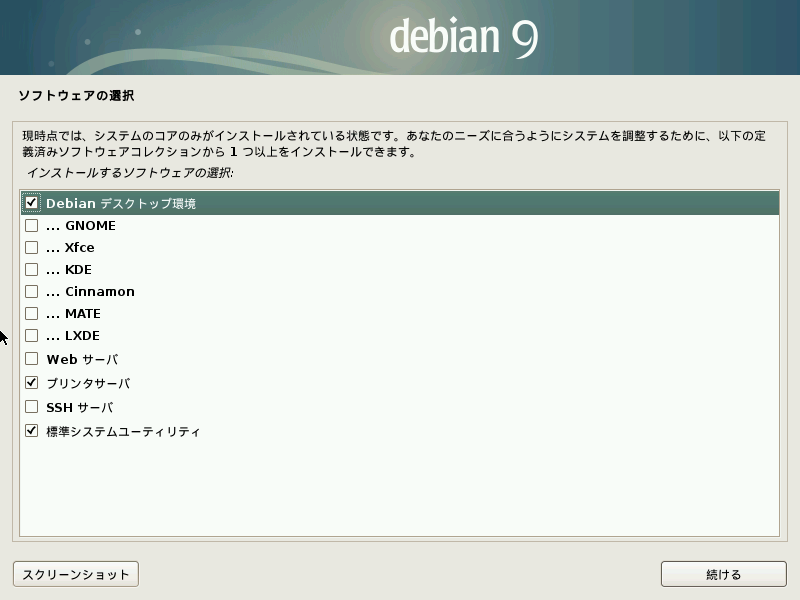
\includegraphics[keepaspectratio,width=1\hsize]{image201907/stretch_tasksel_0.png}
\end{center}

\end{frame}

\begin{frame}{Buster のデフォルトデスクトップ}

\begin{center}
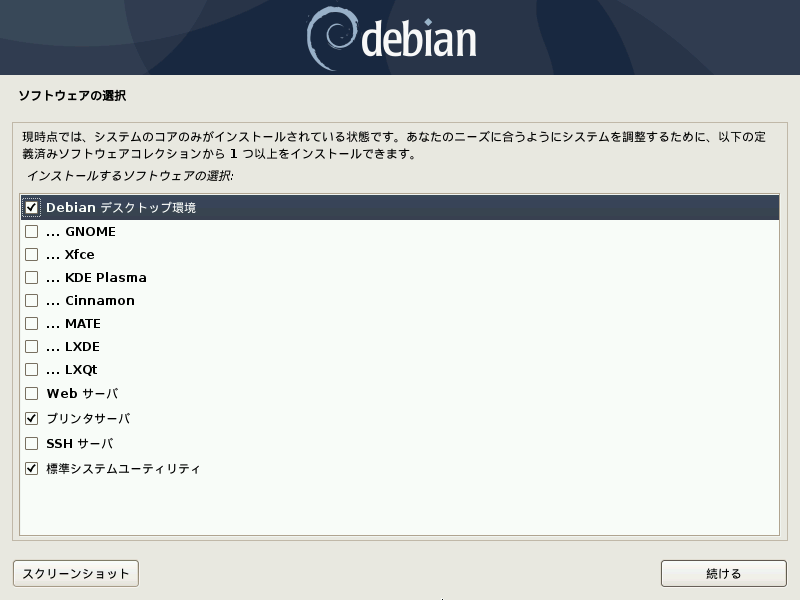
\includegraphics[keepaspectratio,width=1\hsize]{image201907/buster_tasksel_0.png}
\end{center}

\end{frame}

\begin{frame}{Buster のデフォルトデスクトップ}

\begin{center}
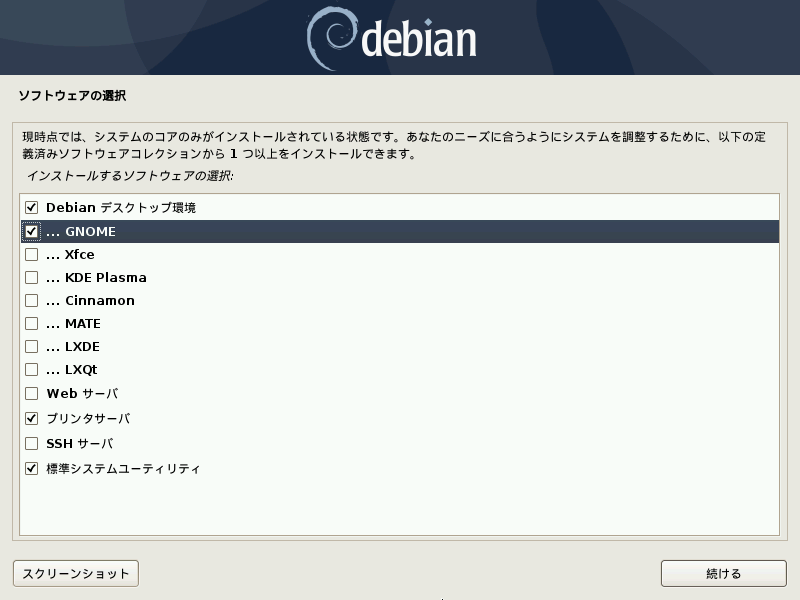
\includegraphics[keepaspectratio,width=1\hsize]{image201907/buster_tasksel_1.png}
\end{center}

\end{frame}

\begin{frame}{Buster のデフォルトデスクトップ}

\begin{center}
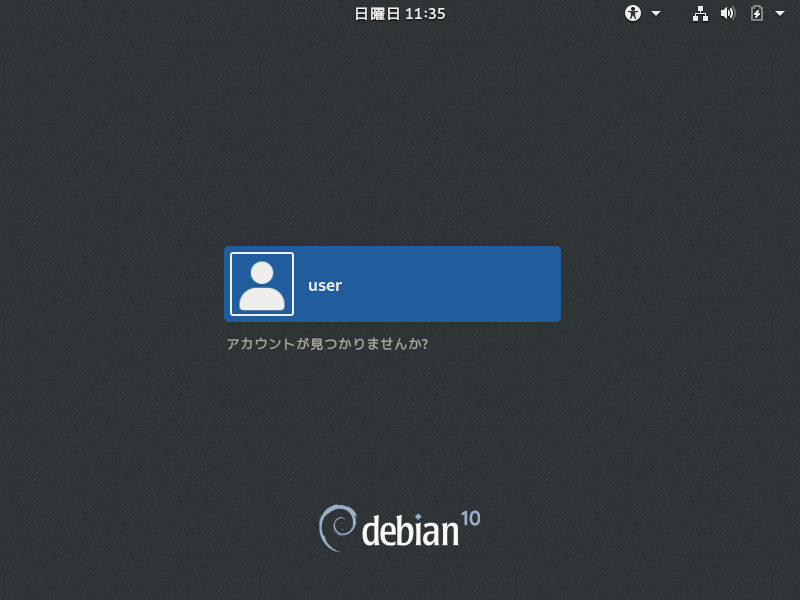
\includegraphics[keepaspectratio,width=1\hsize]{image201907/buster_gdm3.png}
\end{center}

\end{frame}

\begin{frame}{Buster のデフォルトデスクトップ}

\begin{center}
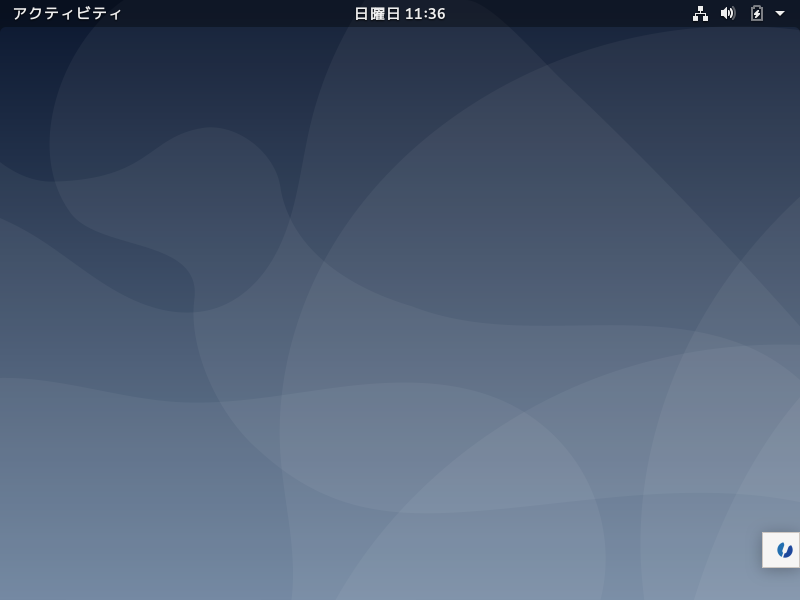
\includegraphics[keepaspectratio,width=1\hsize]{image201907/buster_gnome_1.png}
\end{center}

\end{frame}

\begin{frame}{Buster のデフォルトデスクトップ}

\begin{center}
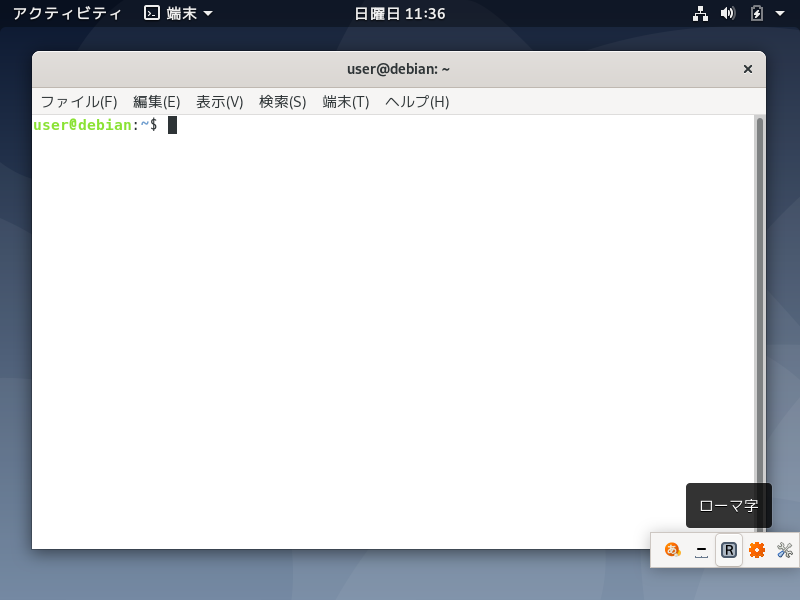
\includegraphics[keepaspectratio,width=1\hsize]{image201907/buster_gnome_2.png}
\end{center}

\end{frame}

\begin{frame}{Buster のデフォルトデスクトップ}

\begin{center}
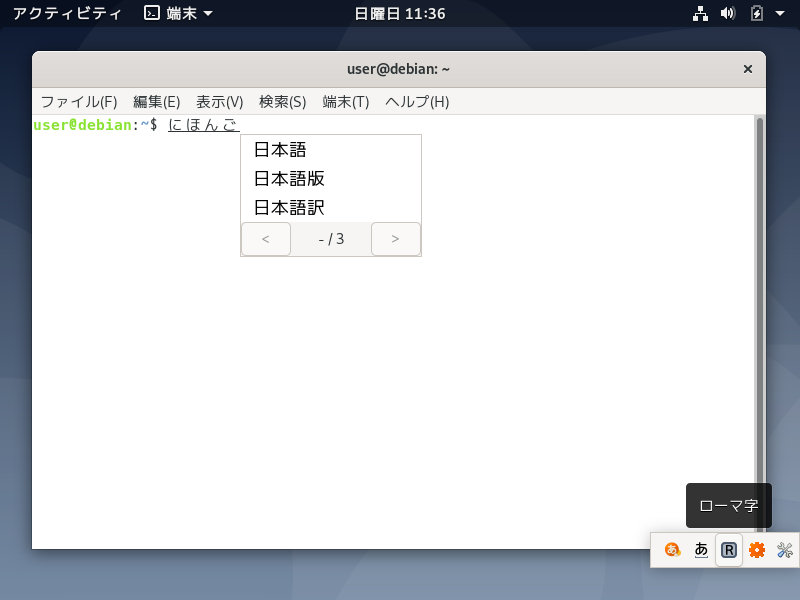
\includegraphics[keepaspectratio,width=1\hsize]{image201907/buster_gnome_3.png}
\end{center}

\end{frame}

\begin{frame}{Stretch のデフォルトデスクトップ}

\begin{center}
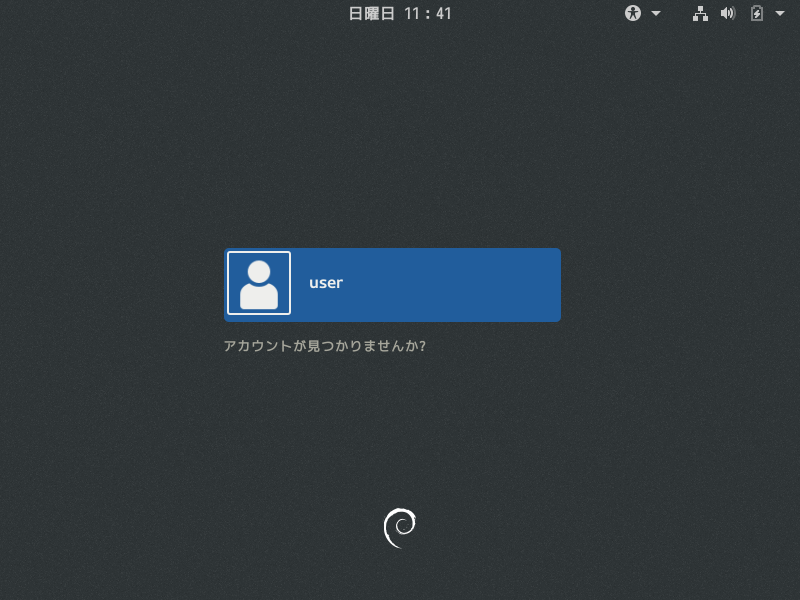
\includegraphics[keepaspectratio,width=1\hsize]{image201907/stretch_gdm3.png}
\end{center}

\end{frame}

\begin{frame}{Stretch のデフォルトデスクトップ}

\begin{center}
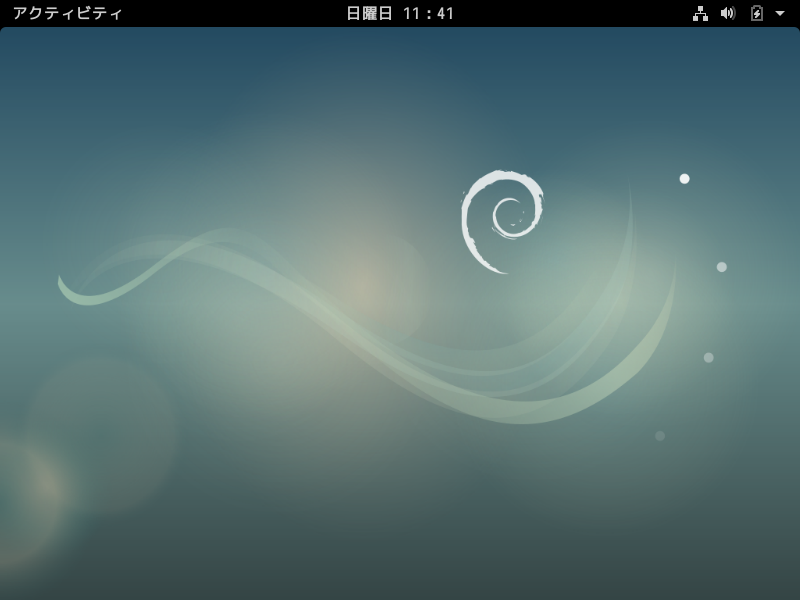
\includegraphics[keepaspectratio,width=1\hsize]{image201907/stretch_gnome_1.png}
\end{center}

\end{frame}

\begin{frame}{Stretch のデフォルトデスクトップ}

\begin{center}
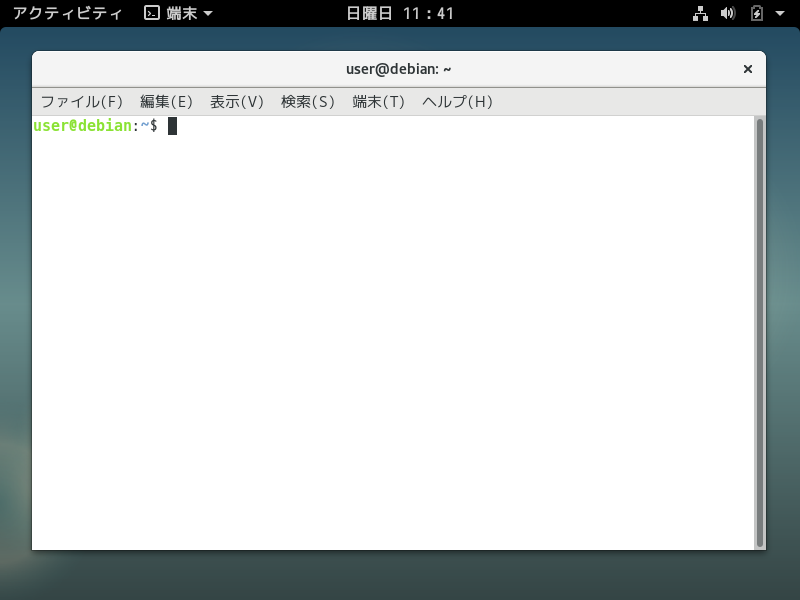
\includegraphics[keepaspectratio,width=1\hsize]{image201907/stretch_gnome_2.png}
\end{center}

\end{frame}

\begin{frame}{Stretch のデフォルトデスクトップ}

\begin{center}
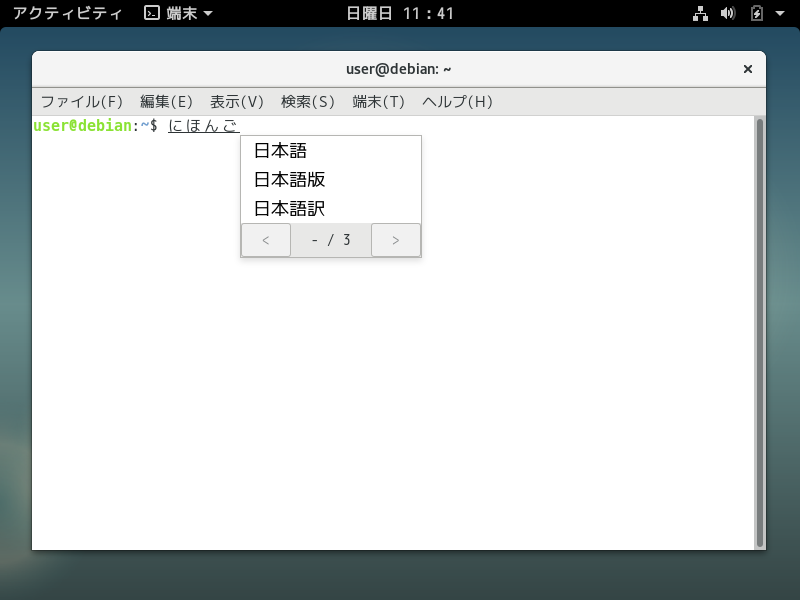
\includegraphics[keepaspectratio,width=1\hsize]{image201907/stretch_gnome_3.png}
\end{center}

\end{frame}

\begin{frame}{Stretch のデフォルトデスクトップ}

\begin{center}
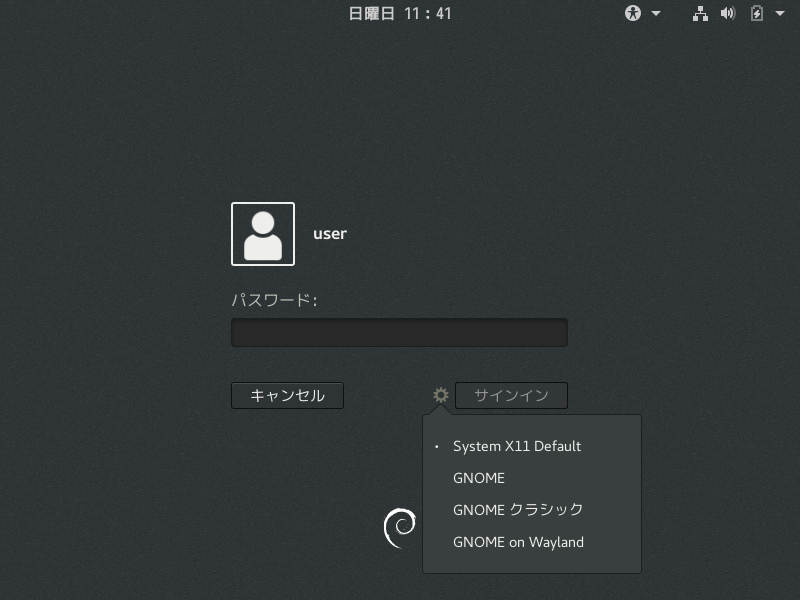
\includegraphics[keepaspectratio,width=1\hsize]{image201907/stretch_gnome_0.png}
\end{center}

\end{frame}

\begin{frame}{Buster のデフォルトデスクトップ}

\begin{center}
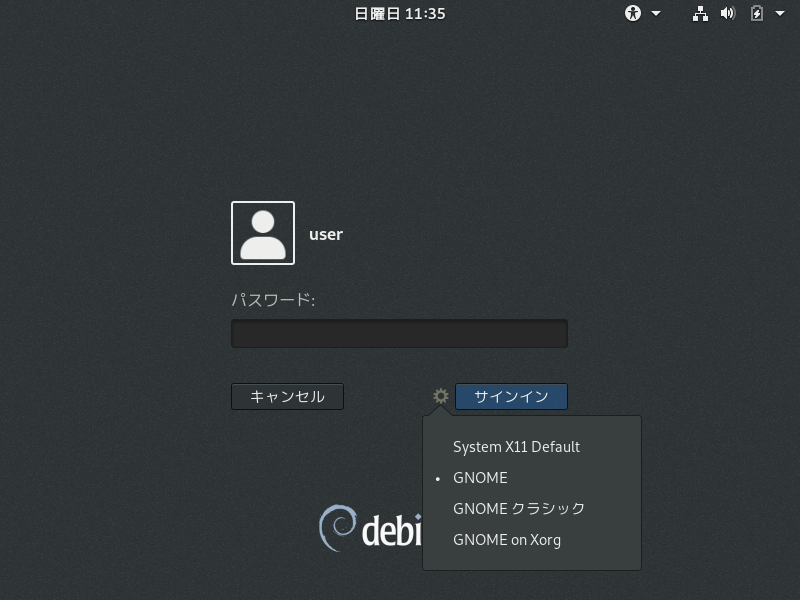
\includegraphics[keepaspectratio,width=1\hsize]{image201907/buster_gnome_0.png}
\end{center}

\end{frame}

\begin{frame}{デフォルトデスクトップ}

\begin{itemize}[<+->]
 \item GNOME
 \item Stretch では GNOME on Xorg
 \item Buster では GNOME on Wayland
\end{itemize}

\end{frame}

\section{Xorg / Wayland}

\begin{frame}{Xorg}

\begin{itemize}
 \item Xセッションでは /etc/X11/Xsession.d/ にあるシェルスクリプトで環境変数などを初期化する
 \item インプットメソッド周りはim-configで
\begin{itemize}
 \item /etc/X11/Xsession.d/70im-config\_launch が設定して、最後に /usr/bin/im-launch がデーモンを起動する
 \item 他の方法(.xsessionrcなど)で設定されたらそれを尊重する
\end{itemize}
\end{itemize}

\end{frame}

\begin{frame}{Wayland (1/2)}

\begin{itemize}[<+->]
 \item Waylandセッションは初期化を扱わない\\
 -- 当然 /etc/X11/Xsession.d/ は使われない
 \item Wayland以外で設定・起動するしかない

\begin{itemize}
 \item 設定方法
\begin{itemize}
 \item systemd -{}-user\\
-- Busterのsystemd ($>= 233$)ではユーザー設定を動的に変えられるようになった(/usr/lib/systemd/user-environment-generators/*)\\
-- 現状gdm3だけはsystemd -{}-user内の変数値を環境変数として取り込む
 \item pam\_env\\
-- 設定が動的に変えられない(設定ファイル /etc/environment などしかない)
 \item ...
\end{itemize}

 \item 起動方法
\begin{itemize}
 \item /etc/xdg/autostart/*.desktop
 \item ...
\end{itemize}

\end{itemize}

\end{itemize}

\end{frame}

\begin{frame}{Wayland (2/2)}
Waylandはウィンドウの位置情報を提供しない\\
\pause
⇒ カーソルの位置がわからない!
\pause
\begin{itemize}
 \item コンポジター(GNOME Shell)の独自APIで実装する\\
(ibus)
\pause
 \item XWayland を使う\\
env GDK\_BACKEND=x11\\
(Busterのim-configでのuim)
\end{itemize}

\end{frame}

\section{Buster}

\begin{frame}{設定}

\begin{itemize}
 \item Xorg では今まで通り設定する
 \item Wayland では別の方法を使う、でも他の方法(.config/environment.d/*.confなど)で設定されたらそれを尊重したい
\end{itemize}
\pause

systemd -{}-user では常にログイン直後に設定される
\pause
\begin{itemize}
 \item 
systemd であれば
\pause
Wayland でも
\pause
Xorg でも
\pause
ssh でも
\pause
区別なく他の方法での設定より前に呼ばれる\\
\pause
⇒これを Wayland で使うなら常に(Xorgであっても)設定するしかない\\
(/usr/lib/systemd/user-environment-generators/70-im-config)
\\
\pause
 \item 
今まで通りの方法など、他で設定されたら尊重したい...\\
⇒ 他の方法で設定されたか後で検出することにする
(IM\_CONFIG\_CHECK\_ENV=1)
\end{itemize}

\end{frame}

\begin{frame}{起動}

\begin{itemize}
 \item Xorg では今まで通り起動する
 \item Wayland では別の方法を使う、でも他の方法で設定されたらそれを尊重することにして起動しない
\end{itemize}
\pause

XDG Autostartはサポートするデスクトップ環境では常に起動されるが、WaylandかXorgか区別は可能\\
\pause
⇒ WaylandのときのみXDG Autostartで起動するようにする\\
(/etc/xdg/autostart/im-launch.desktop)

\end{frame}

\section{まとめ}

\begin{frame}{まとめ}
\begin{itemize}
 \item BusterではGNOME Waylandがデフォルトデスクトップで、日本語入力できるようにした
 \item WaylandではXorgのスクリプトが一切実行されない
 \item Busterの gdm3 + GNOME Wayland ではsystemdのuser-environment-generatorとXDG Autostartを使うようにした
 \item systemd + gdm3 + GNOME Wayland の組み合わせ以外では動作しない
\end{itemize}

\end{frame}

\end{document}


;;; Local Variables: ***
;;; outline-regexp: "\\([ 	]*\\\\\\(documentstyle\\|documentclass\\|emtext\\|section\\|begin{frame}\\)\\*?[ 	]*[[{]\\|[]+\\)" ***
;;; End: ***
